% Toolbar icon: linear → quadratic — a linear triangle (3 corner nodes), an
% arrow, and the same triangle upgraded to quadratic (corner + mid-edge nodes).
\documentclass[tikz,border=2mm]{standalone}
\usetikzlibrary{arrows.meta,calc,shapes.geometric}
\begin{document}
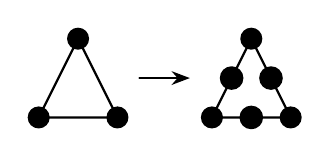
\begin{tikzpicture}[line width=1.3pt, line cap=round, line join=round, >=Stealth, x=1mm,y=1mm]
  % --- linear triangle (corner nodes only) ---
  \coordinate (A) at (-16,-5);
  \coordinate (B) at (-6,-5);
  \coordinate (C) at (-11,5);
  \draw[thick] (A) -- (B) -- (C) -- cycle;
  \fill (A) circle (1.4);
  \fill (B) circle (1.4);
  \fill (C) circle (1.4);
  % --- arrow ---
  \draw[thick,->] (-3.2,0) -- (3.2,0);
  % --- quadratic triangle (corner + mid-edge nodes) ---
  \coordinate (D) at (6,-5);
  \coordinate (E) at (16,-5);
  \coordinate (F) at (11,5);
  \draw[thick] (D) -- (E) -- (F) -- cycle;
  \fill (D) circle (1.4);
  \fill (E) circle (1.4);
  \fill (F) circle (1.4);
  \fill ($(D)!0.5!(E)$) circle (1.5);
  \fill ($(E)!0.5!(F)$) circle (1.5);
  \fill ($(F)!0.5!(D)$) circle (1.5);
\end{tikzpicture}
\end{document}
